\chapter{A energia cinética e a segurança no trânsito}\label{ch:g9:kinetic-energy-safety}

Desde os brinquedos de corda da sua infância, a \omterm{def:g5:everyday-energy:energy}{energia} foi uma
história de reservas e formas --- viva, útil e sem números. A espera
acaba agora. A \omterm{def:g5:everyday-energy:energy}{energia} do movimento ganha a fórmula dela, a \omterm{def:g5:everyday-energy:energy}{energia}
ganha a \omterm{def:g6:measurement-in-science:measuring}{unidade} dela, e a aritmética acaba governando um assunto de
vida ou morte: por que um carro ao dobro da \omterm{def:g7:motion-average-speed:formula}{velocidade} é quatro vezes
mais difícil de parar, e quanto um único segundo de desatenção custa
em \omterm{def:g2:measuring-length:units}{metros}.

\section{A energia do movimento}

\begin{definition}[O joule]\label{def:g9:kinetic-energy-safety:joule}
A \omterm{def:g5:everyday-energy:energy}{energia} --- em todas as formas dela --- é medida em
\emph{joules}\index{joule} (\unit{J}), em homenagem ao experimentador
que provou que o próprio \omterm{def:g5:heat-and-insulation:heat}{calor} é uma forma de \omterm{def:g5:everyday-energy:energy}{energia}. Âncoras:
levantar este livro do chão até a prateleira gasta uns poucos joules;
um coração batendo, cerca de um joule por batida; uma barra de
chocolate guarda um milhão de joules de \omterm{def:g5:everyday-energy:energy}{energia} alimentar.
\end{definition}

\begin{proposition}[A energia cinética]\label{prop:g9:kinetic-energy-safety:formula}
Um corpo de \omterm{def:g3:measuring-mass:mass}{massa} $m$ (em \unit{kg}) que se move com \omterm{def:g7:motion-average-speed:formula}{velocidade} $v$
(em \unit{m/s}) carrega, em virtude do movimento dele, a
\emph{energia cinética}\index{energia cinética}
\[
E_k = \frac{1}{2} \times m \times v^2 ,
\]
em \omterm{def:g9:kinetic-energy-safety:joule}{joules}. Dois botões, expoentes desiguais: dobrar a \omterm{def:g3:measuring-mass:mass}{massa} dobra
$E_k$ --- mas dobrar a \emph{\omterm{def:g7:motion-average-speed:formula}{velocidade}} a \emph{quadruplica}, pois a
\omterm{def:g7:motion-average-speed:formula}{velocidade} entra ao quadrado. A \omterm{def:g7:motion-average-speed:formula}{velocidade} é o botão perigoso.
\end{proposition}

\begin{example}[Primeiros cálculos]\label{ex:g9:kinetic-energy-safety:first}
Uma bola de futebol de \qty{0.45}{kg} a \qty{20}{m/s}:
$E_k = 0.5 \times 0.45 \times 20^2 = \qty{90}{J}$. Um velocista de
\qty{60}{kg} a \qty{10}{m/s}:
$0.5 \times 60 \times 100 = \qty{3000}{J}$. Um carro de
\qty{1000}{kg} a \qty{50}{km/h} --- converta primeiro:
$50 \div 3.6 \approx \qty{13.9}{m/s}$ ---
$E_k = 0.5 \times 1000 \times 13.9^2 \approx \qty{9.7e4}{J}$: quase
cem mil \omterm{def:g9:kinetic-energy-safety:joule}{joules}. O mesmo carro a \qty{100}{km/h}: quatro vezes mais
--- \qty{3.9e5}{J}. O aviso da fórmula, em números.
\end{example}

\begin{omfigure}
\begin{tikzpicture}
\begin{axis}[omaxis, width=10.2cm, height=6.0cm,
    xlabel={velocidade $v$ (\unit{km/h})},
    ylabel={$E_k$ (\unit{kJ})},
    xtick={0,30,50,70,90,110,130}, ytick={0,100,200,300,400,500},
    ymin=0, ymax=560, xmin=0, xmax=140, samples=100]
  \addplot[very thick, omThm, domain=0:135]
    {0.5*1000*(x/3.6)^2/1000};
  \addplot[only marks, mark=*, omDef] coordinates
    {(50,96.5) (100,385.8)};
  \node[right, font=\small, omDef] at (axis cs:38,130)
    {\qty{50}{km/h}};
  \node[left, font=\small, omDef] at (axis cs:99,400)
    {\qty{100}{km/h}: o quádruplo};
\end{axis}
\end{tikzpicture}

{\small A \omterm{prop:g9:kinetic-energy-safety:formula}{energia cinética} de um carro de uma tonelada contra a
\omterm{def:g7:motion-average-speed:formula}{velocidade}: não uma reta, mas uma parábola --- o quadrado da fórmula,
desenhado. Dobre a \omterm{def:g7:motion-average-speed:formula}{velocidade}, quadruplique a \omterm{def:g5:everyday-energy:energy}{energia} da qual é
preciso se livrar.}
\end{omfigure}

\begin{example}[Para onde a frenagem a manda]\label{ex:g9:kinetic-energy-safety:brakes}
Para parar, um carro precisa entregar a $E_k$ inteira dele a alguma
coisa --- a \omterm{def:g5:everyday-energy:energy}{energia} é repassada, nunca apagada, como as correntes da
sua infância insistiam. A garra dos freios a converte em \omterm{def:g5:heat-and-insulation:heat}{calor}: os
discos brilham em âmbar depois das descidas de montanha, e o cheiro
de freio quente \emph{é} \omterm{prop:g9:kinetic-energy-safety:formula}{energia cinética} se aposentando. Numa
batida, a entrega é violenta e instantânea --- para dentro do aço
amassado. Todo número de segurança viária adiante é essa
contabilidade: quanto maior a $E_k$, mais longa, ou mais feia, a
aposentadoria dela.
\end{example}

\begin{omfigure}
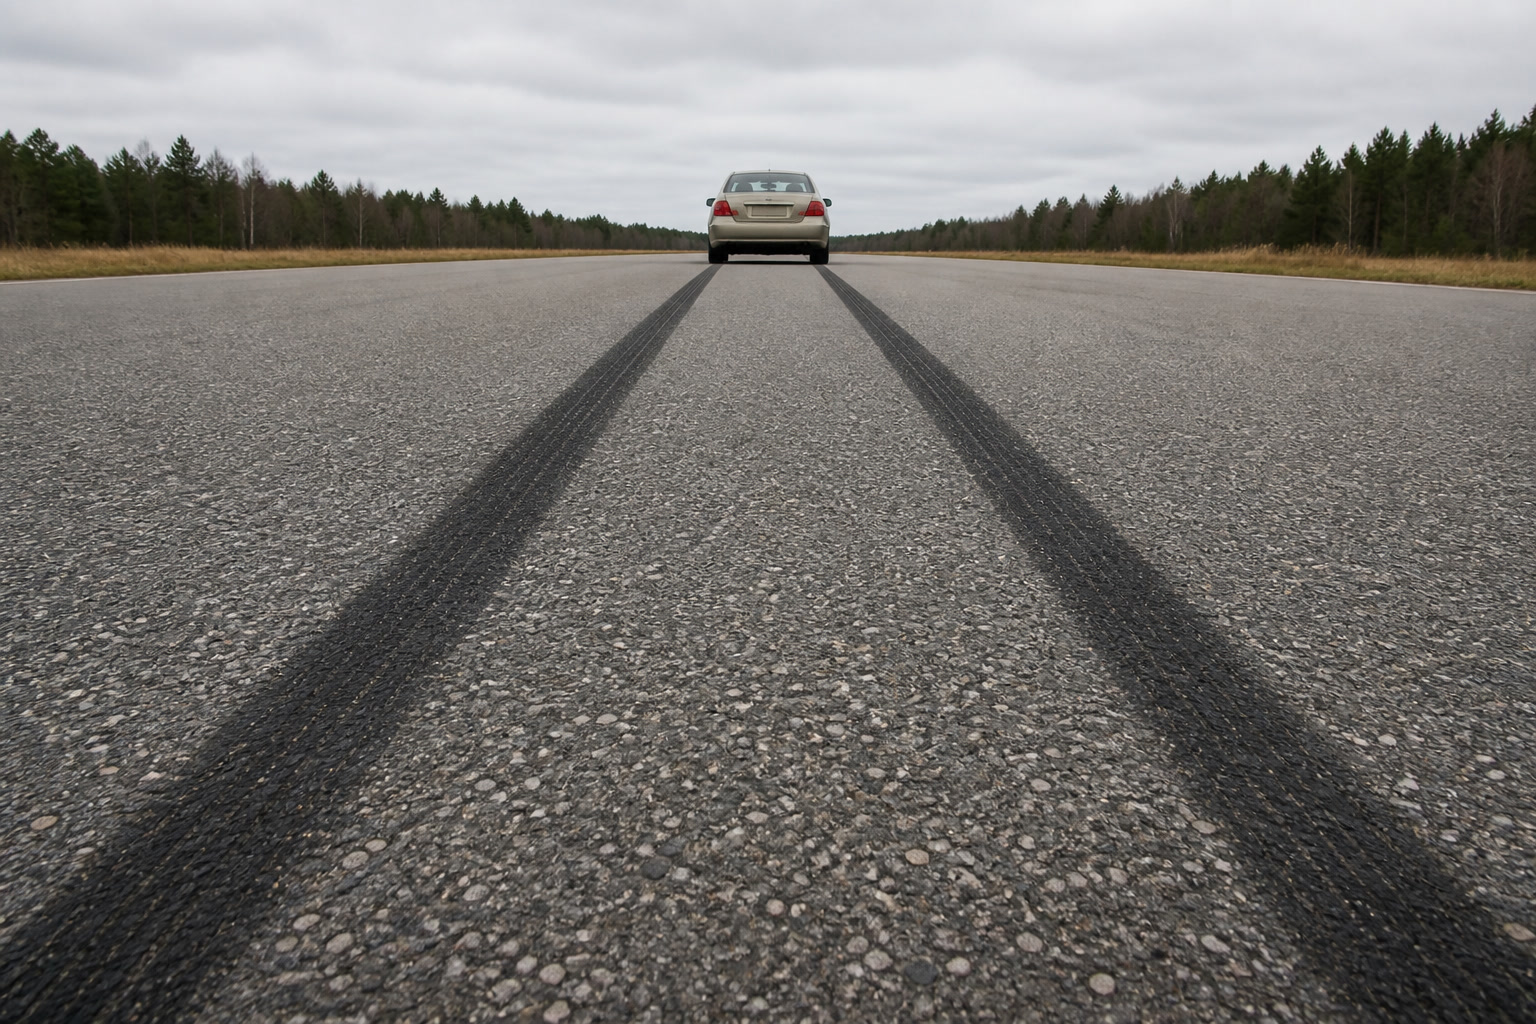
\includegraphics[width=0.55\linewidth]{images/book1/ai/g9-kinetic-skid-marks.jpg}

{\small Para onde foi a \omterm{prop:g9:kinetic-energy-safety:formula}{energia cinética}: os freios e a estrada a transformaram em \omterm{def:g5:heat-and-insulation:heat}{calor}, e os pneus assinaram o recibo.}
\end{omfigure}

\section{A distância de parada}

\begin{proposition}[Parar = pensar + frear]\label{prop:g9:kinetic-energy-safety:stopping}
Um motorista que enxerga o perigo só para depois de dois trechos de
estrada:
\begin{enumerate}
  \item a \emph{distância de reação}\index{distância de reação}: a
        estrada percorrida enquanto o cérebro percebe e o pé se move
        --- cerca de um segundo inteiro na \omterm{def:g7:motion-average-speed:formula}{velocidade} sem mudança, e
        por isso esse trecho cresce \emph{em proporção} a $v$;
  \item a \emph{distância de frenagem}\index{distância de frenagem}:
        a estrada de que os freios precisam para aposentar a \omterm{prop:g9:kinetic-energy-safety:formula}{energia
        cinética} --- e, como $E_k$ carrega $v^2$, esse trecho cresce
        com o \emph{quadrado} da \omterm{def:g7:motion-average-speed:formula}{velocidade}: \omterm{def:g7:motion-average-speed:formula}{velocidade} dobrada,
        estrada de frenagem quadruplicada.
\end{enumerate}
A soma dos dois, a \emph{distância de parada}, é o número que
encontra a criança correndo atrás da bola.
\end{proposition}

\begin{example}[A tabela que todo motorista deveria ter]\label{ex:g9:kinetic-energy-safety:table}
Estrada seca, motorista atento (um segundo de reação; freios bons):
\begin{center}
\begin{tabular}{l|c|c|c}
\omterm{def:g7:motion-average-speed:formula}{velocidade} & reação & frenagem & parada \\
\hline
\qty{50}{km/h} & \qty{14}{m} & \qty{13}{m} & \qty{27}{m} \\
\qty{90}{km/h} & \qty{25}{m} & \qty{40}{m} & \qty{65}{m} \\
\qty{130}{km/h} & \qty{36}{m} & \qty{85}{m} & \qty{121}{m}
\end{tabular}
\end{center}
Leia duas vezes. Na \omterm{def:g7:motion-average-speed:formula}{velocidade} da cidade, um ônibus e meio; na
\omterm{def:g7:motion-average-speed:formula}{velocidade} da estrada, uma pista de atletismo inteira e mais um
quinto. E as proporções confirmam as duas leis: a reação cresce como
$v$, a frenagem como $v^2$ --- em alta \omterm{def:g7:motion-average-speed:formula}{velocidade}, a frenagem devora
o total.
\end{example}

\begin{method}[Estimar uma distância de parada]\label{met:g9:kinetic-energy-safety:estimate}
\begin{enumerate}
  \item converta a \omterm{def:g7:motion-average-speed:formula}{velocidade} para \unit{m/s} (divida os \unit{km/h}
        por $3.6$);
  \item \omterm{prop:g9:kinetic-energy-safety:stopping}{distância de reação}: a viagem de um segundo --- o próprio
        número em \unit{m/s}, em \omterm{def:g2:measuring-length:units}{metros};
  \item \omterm{prop:g9:kinetic-energy-safety:stopping}{distância de frenagem}: escale uma âncora conhecida pelo
        quadrado --- a partir dos \qty{13}{m} a \qty{50}{km/h},
        multiplique por $(v/50)^2$;
  \item some, e compare com o que a estrada à frente de fato oferece.
\end{enumerate}
Estradas molhadas dobram a parcela da frenagem; motoristas cansados
ou distraídos esticam o segundo de reação na direção de dois ---
refaça a soma com as entradas honestas.
\end{method}

\begin{example}[O preço de uma olhadinha]\label{ex:g9:kinetic-energy-safety:glance}
Uma olhadinha de dois segundos no celular a \qty{90}{km/h}: o carro
percorre $2 \times 25 = \qty{50}{m}$ --- meio campo de futebol ---
dirigido às cegas, antes mesmo de qualquer segundo de reação começar.
Na \omterm{def:g7:motion-average-speed:formula}{velocidade} da cidade, a mesma olhadinha gasta às cegas
\qty{28}{m}: passa do cruzamento, passa do portão da escola. O
componente mais perigoso do carro não é medido por fórmula nenhuma
aqui: a atenção de quem dirige.
\end{example}

\begin{remark}[Cintos, bolsas de ar e capacetes]\label{rem:g9:kinetic-energy-safety:belts}
Numa colisão, o carro para em um \omterm{def:g2:measuring-length:units}{metro} de amassamento --- mas um
passageiro sem cinto continua na \omterm{def:g7:motion-average-speed:formula}{velocidade} inteira (a frase discreta
do capítulo passado, aplicada com crueza) até ser parado pelo que
vier: painel, para-brisa, asfalto. Os cintos de segurança e as bolsas
de \omterm{def:g2:air-around-us:air}{ar} param o corpo ao longo de uma distância e de um tempo maiores,
aposentando a \omterm{prop:g9:kinetic-energy-safety:formula}{energia cinética} dele com delicadeza em vez de tudo de
uma vez; o capacete do ciclista faz o mesmo pelo conteúdo
insubstituível do crânio, com a espuma amassável dele comprando
\omterm{def:g2:measuring-length:units}{centímetros} de parada suave. Nenhum deles reduz a sua $E_k$ em um
\omterm{def:g9:kinetic-energy-safety:joule}{joule} que seja --- eles civilizam a aposentadoria dela.
\end{remark}

\section{Exercícios}

\begin{exercise}[$\star$]\label{exo:g9:kinetic-energy-safety:1}
Dê a \omterm{def:g6:measurement-in-science:measuring}{unidade} de \omterm{def:g5:everyday-energy:energy}{energia} e duas âncoras dela, e escreva a fórmula da
\omterm{prop:g9:kinetic-energy-safety:formula}{energia cinética} com as \omterm{def:g6:measurement-in-science:measuring}{unidades}.
\end{exercise}

\begin{exercise}[$\star$]\label{exo:g9:kinetic-energy-safety:2}
Calcule $E_k$: uma lebre de \qty{2}{kg} a \qty{10}{m/s}; um jogador
de rúgbi de \qty{80}{kg} a \qty{5}{m/s}.
\end{exercise}

\begin{exercise}[$\star$]\label{exo:g9:kinetic-energy-safety:3}
O que aumenta mais a $E_k$ de um carro: acrescentar metade da \omterm{def:g3:measuring-mass:mass}{massa}
dele em carga, ou aumentar a \omterm{def:g7:motion-average-speed:formula}{velocidade} dele em metade? Mostre os
dois fatores.
\end{exercise}

\begin{exercise}[$\star$]\label{exo:g9:kinetic-energy-safety:4}
Diga os nomes dos dois trechos da distância de parada e as leis de
crescimento deles --- uma proporcional, uma ao quadrado.
\end{exercise}

\begin{exercise}[$\star$]\label{exo:g9:kinetic-energy-safety:5}
Pela tabela do motorista: que fração da distância de parada é
frenagem a \qty{50}{km/h} --- e a \qty{130}{km/h}? O que mudou?
\end{exercise}

\begin{exercise}[$\star$]\label{exo:g9:kinetic-energy-safety:6}
Para onde vai a \omterm{prop:g9:kinetic-energy-safety:formula}{energia cinética} de um carro que freia? Cite o cheiro
e o brilho --- e a lei da infância que proíbe que ela simplesmente
suma.
\end{exercise}

\begin{exercise}[$\star$]\label{exo:g9:kinetic-energy-safety:7}
Calcule a \omterm{prop:g9:kinetic-energy-safety:stopping}{distância de reação} a \qty{36}{km/h}, \qty{72}{km/h} e
\qty{108}{km/h} (um segundo de motorista atento). Que padrão simples
as respostas seguem?
\end{exercise}

\begin{exercise}[$\star$]\label{exo:g9:kinetic-energy-safety:8}
Por que um cinto de segurança não reduz a sua \omterm{prop:g9:kinetic-energy-safety:formula}{energia cinética} --- e
o que ele civiliza em vez disso?
\end{exercise}

\begin{exercise}[$\star\star$]\label{exo:g9:kinetic-energy-safety:9}
A \omterm{prop:g9:kinetic-energy-safety:stopping}{distância de frenagem} de uma motoneta é de \qty{8}{m} a
\qty{30}{km/h}. Estime-a a \qty{60}{km/h} e a \qty{90}{km/h} --- e
enuncie a lei pela qual você escalou.
\end{exercise}

\begin{exercise}[$\star\star$]\label{exo:g9:kinetic-energy-safety:10}
As prefeituras baixam os limites em zona escolar de \qty{50}{} para
\qty{30}{km/h}. Compare as duas distâncias de parada (âncora:
\qty{13}{m} de frenagem a $50$; um segundo de reação) --- e as duas
\omterm{prop:g9:kinetic-energy-safety:formula}{energias cinéticas}. Qual comparação você acha mais persuasiva num
cartaz?
\end{exercise}

\begin{exercise}[$\star\star$]\label{exo:g9:kinetic-energy-safety:11}
A chuva dobra as \omterm{prop:g9:kinetic-energy-safety:stopping}{distâncias de frenagem}. Reconstrua a coluna de
parada da tabela do motorista para estrada molhada a $50$ e
\qty{90}{km/h} --- que componente você dobrou, qual não, e por quê?
\end{exercise}

\begin{exercise}[$\star\star\star$]\label{exo:g9:kinetic-energy-safety:12}
Um caminhão de \qty{20000}{kg} rola a \qty{90}{km/h}. Calcule a $E_k$
dele em notação científica; ache a \omterm{def:g7:motion-average-speed:formula}{velocidade} com que um carro de
\qty{1000}{kg} igualaria essa \omterm{def:g5:everyday-energy:energy}{energia} (iguale as duas fórmulas --- a
álgebra é sua neste ano); e conclua por que existem rampas de escape
para caminhões desgovernados nas estradas de montanha, enquanto rampa
nenhuma dessas serve aos carros.
\end{exercise}

\section{Problema: A campanha de segurança}

\begin{problem}[{Problema de fim de semana --- a turma projeta a
campanha de segurança no trânsito da cidade; cartazes conferidos por
fórmula; as perguntas difíceis do
prefeito}]\label{pb:g9:kinetic-energy-safety:1}
A cidade encomenda uma campanha, com uma condição: todo número de
todo cartaz precisa sobreviver a uma auditoria de física. A turma
calcula. (Âncoras: reação de um segundo; frenagem de \qty{13}{m} a
\qty{50}{km/h}, escalando pelo quadrado; \omterm{def:g3:measuring-mass:mass}{massa} do carro
\qty{1000}{kg}.)

\medskip\noindent\textbf{Parte I --- Cartaz um: ``50 e não 60''.}
\begin{enumerate}
  \item Calcule as duas \omterm{def:g7:motion-average-speed:formula}{velocidades} em \unit{m/s} (uma casa decimal).
  \item As \omterm{prop:g9:kinetic-energy-safety:stopping}{distâncias de reação} nas duas \omterm{def:g7:motion-average-speed:formula}{velocidades}?
  \item As \omterm{prop:g9:kinetic-energy-safety:stopping}{distâncias de frenagem} nas duas (escale a âncora)?
  \item A manchete do cartaz: ``Dez \omterm{def:g6:measurement-in-science:measuring}{unidades} a mais de \omterm{def:g7:motion-average-speed:formula}{velocidade},
        --- quantos \omterm{def:g2:measuring-length:units}{metros} a mais de parada?'' Preencha o número.
\end{enumerate}

\medskip\noindent\textbf{Parte II --- Cartaz dois: ``O muro da
\omterm{def:g7:motion-average-speed:formula}{velocidade}''.}
O projeto mostra as \omterm{def:g5:everyday-energy:energy}{energias} de colisão como alturas de queda: uma
batida na \omterm{def:g7:motion-average-speed:formula}{velocidade} $v$ ``equivale'' a cair da altura em que a mesma
\omterm{def:g5:everyday-energy:energy}{energia} seria ganha.
\begin{enumerate}[resume]
  \item Calcule a $E_k$ do carro a \qty{50}{km/h} (da Parte I) e a
        \qty{90}{km/h}.
  \item Os artistas precisam de alturas: cair de \qty{1}{m} rende
        cerca de \qty{9.8}{kJ} para esse carro ($m g h$ --- a outra
        fórmula do próximo capítulo, emprestada mais cedo). A que
        alturas de queda correspondem as duas \omterm{def:g5:everyday-energy:energy}{energias} de colisão?
        (Divida; arredonde para o \omterm{def:g2:measuring-length:units}{metro}.)
  \item Que prédios do dia a dia correspondem a essas alturas?
        Rascunhe a frase do cartaz.
  \item O prefeito objeta: ``Ninguém dirige contra muros; os carros
        amassam, os cintos seguram.'' Defenda a física do cartaz
        concedendo o ponto dele --- o que as zonas de deformação e os
        cintos mudam, e que número eles não mudam?
\end{enumerate}

\medskip\noindent\textbf{Parte III --- Cartaz três: ``Um segundo''.}
\begin{enumerate}[resume]
  \item A \qty{90}{km/h}, quantos \omterm{def:g2:measuring-length:units}{metros} um segundo distraído custa
        antes de qualquer frenagem? E uma olhadinha de dois segundos
        no celular?
  \item A variante do motorista cansado: reação esticada para dois
        segundos. Recalcule a distância de parada completa a
        \qty{90}{km/h} e compare com os \qty{65}{m} do motorista
        atento.
  \item Um vereador cético: ``Certamente um segundo importa pouco ao
        lado daqueles números grandes de frenagem.'' Em que
        \omterm{def:g7:motion-average-speed:formula}{velocidades} ele está mais errado --- baixas ou altas?
        (Compare as leis de crescimento dos dois componentes.)
  \item Assine a campanha: três frases de rodapé de cartaz, uma por
        cartaz, cada uma carregando a fórmula dela em palavras
        simples.
\end{enumerate}
\end{problem}
